%! Author = Omar Iskandarani
%! Title = Swirl String Theory (SST) Canon v0.5
%! Date = Sept 4, 2025
%! Affiliation = Independent Researcher, Groningen, The Netherlands
%! License = © 2025 Omar Iskandarani. All rights reserved. This manuscript is made available for academic reading and citation only. No republication, redistribution, or derivative works are permitted without explicit written permission from the author. Contact: info@omariskandarani.com
%! ORCID = 0009-0006-1686-3961
%! DOI = 10.5281/zenodo.17155854

\newcommand{\paperversion}{\textbf{v0.0.1}} % Semantic versioning: vMAJOR.MINOR.PATCH
\newcommand{\papertitle}{Long-Distance Swirl Gravity from Chiral Swirling Knots with Central Holes}
\newcommand{\paperdoi}{10.5281/zenodo.17155854}

%========================================================================================
% PACKAGES AND DOCUMENT CONFIGURATION
%========================================================================================
\documentclass[reprint,aps,onecolumn,nofootinbib]{revtex4-2}

% ====== minimal packages ======
\usepackage{amsmath,amssymb,amsfonts}
\usepackage{bm}
\usepackage{physics}
\usepackage{microtype}
\usepackage{tcolorbox}
\usepackage{hyperref}
\hypersetup{colorlinks=true,linkcolor=blue,citecolor=blue,urlcolor=blue}

% ==== Packages ====
\usepackage[T1]{fontenc}
\usepackage{lmodern}
\usepackage{booktabs}
\usepackage[utf8]{inputenc}
\usepackage[caption=false]{subfig} % REVTeX-compatible

% ===== Gauge sector macros =====
\renewcommand{\Tr}{\mathrm{Tr}}
\newcommand{\ii}{\mathrm{i}}
% Gauge fields (adjoints; indices a=1..8, i=1..3)
\newcommand{\GsA}{G^a_{\mu\nu}}
\newcommand{\WsI}{W^i_{\mu\nu}}
\newcommand{\Bmn}{B_{\mu\nu}}

% ===============================
% Macros (canonicalized)
% ===============================

% swirl arrows (context-aware)
\newcommand{\swirlarrow}{%
    \mathchoice{\mkern-2mu\scriptstyle\boldsymbol{\circlearrowleft}}%
    {\mkern-2mu\scriptstyle\boldsymbol{\circlearrowleft}}%
    {\mkern-2mu\scriptscriptstyle\boldsymbol{\circlearrowleft}}%
    {\mkern-2mu\scriptscriptstyle\boldsymbol{\circlearrowleft}}%
}
\newcommand{\swirlarrowcw}{%
    \mathchoice{\mkern-2mu\scriptstyle\boldsymbol{\circlearrowright}}%
    {\mkern-2mu\scriptstyle\boldsymbol{\circlearrowright}}%
    {\mkern-2mu\scriptscriptstyle\boldsymbol{\circlearrowright}}%
    {\mkern-2mu\scriptscriptstyle\boldsymbol{\circlearrowright}}%
}

% Canonical symbols
\newcommand{\vswirl}{\mathbf{v}_{\swirlarrow}}
\newcommand{\vswirlcw}{\mathbf{v}_{\swirlarrowcw}}
\newcommand{\SwirlClock}{S_{(t)}^{\swirlarrow}}
\newcommand{\SwirlClockcw}{S_{(t)}^{\swirlarrowcw}}
\newcommand{\omegas}{\boldsymbol{\omega}_{\swirlarrow}}  % swirl vorticity
\newcommand{\vscore}{v_{\swirlarrow}}                    % shorthand: |v_swirl| at r=r_c
\newcommand{\vnorm}{\lVert \vswirl \rVert}               % swirl speed magnitude
\newcommand{\rhof}{\rho_{\!f}}                           % effective fluid density
\newcommand{\rhoE}{\rho_{\!E}}                           % swirl energy density
\newcommand{\rhom}{\rho_{\!m}}                           % mass-equivalent density
\newcommand{\rc}{r_c}                                    % string core radius (swirl string radius)
\newcommand{\FmaxEM}{F_{\mathrm{EM}}^{\max}}             % EM-like maximal force scale
\newcommand{\FmaxG}{F_{\mathrm{G}}^{\max}}               % G-like maximal force scale
\newcommand{\Lam}{\Lambda}                               % Swirl Coulomb constant
\newcommand{\Om}{\Omega_{\swirlarrow}}                   % swirl angular frequency profile
\newcommand{\alpg}{\alpha_g}                             % gravitational fine-structure analogue
% --- Minimal macro prelude (safe, local) ---
\providecommand{\rc}{r_c}
\newcommand{\omegaVec}{\boldsymbol{\omega}}
\newcommand{\rhoF}{\rho_{\!f}}     % effective fluid density
\newcommand{\rhoM}{\rho_{\!m}}     % mass-equivalent density
\newcommand{\OmegaCore}{\Omega_{\mathrm{core}}}
\newcommand{\bg}{\mathrm{bg}}
\newcommand{\core}{\mathrm{core}}
\newcommand{\GammaC}{\Gamma_C}

% ===============================
% Policy: the golden constant is only allowed via hyperbolic functions.
\newcommand{\xig}{\operatorname{asinh}\!\left(\tfrac{1}{2}\right)}
\newcommand{\phig}{\exp(\xig)}
\newcommand{\phialg}{\bigl(1+\sqrt{5}\bigr)/2}
\newcommand{\xigold}{\tfrac{3}{2}\,\xig}
\newcommand{\GoldenDeclare}{%
    \textbf{Golden (hyperbolic)}:\ \(\ln\phi=\xig\), hence \(\phi=\phig\).
    \ \emph{(Equivalently, \(\phi=\phialg\); the algebraic form is derivative.)}%
}
\usepackage{graphicx}
\usepackage{geometry}
\geometry{margin=1in}

% Macros (explicit, macro-free chat-safe)

% --- Add to your preamble (if not already present) ---
%-------------------------------------------
% Put this in your preamble (once)
%-------------------------------------------
\usepackage{tikz}
\usetikzlibrary{calc,arrows.meta,decorations.markings,decorations.pathmorphing}

% A tiny style for loop arrows
\tikzset{
    looparrow/.style={-{Stealth[length=2.5mm,width=1.8mm]},thick},
    knotline/.style={ultra thick, blue!70},
    testloopON/.style={thick, draw=green!60!black},
    testloopOFF/.style={thick, draw=red!70},
    axes/.style={very thick, black},
}

\usepackage{siunitx}
\AtBeginDocument{\RenewCommandCopy\qty\SI}

% Styling helpers
\tikzset{
    axisline/.style={very thick, black},
    corecircle/.style={thick, dashed, gray},
    knotline/.style={ultra thick, blue!65},
    swirlarrow/.style={-{Stealth[length=3mm,width=2mm]}, thick},
    vline/.style={-{Stealth[length=3mm,width=2mm]}, thick, teal!70!black},
    tube/.style={line width=6pt, line cap=round},
    ghost/.style={opacity=0.25},
    labelbox/.style={fill=white, inner sep=2pt, rounded corners=2pt},
}

\usetikzlibrary{knots,hobby,calc,intersections,decorations.pathreplacing,shapes.geometric,spath3}

% ------- Shared styles (from your preamble) -------
\tikzset{
    knot diagram/every strand/.append style={
        line cap=round,
        line join=round,
        ultra thick,
        red
    },
    every knot/.style={line cap=round,line join=round,very thick},
    strand/.style={line cap=round,line join=round,line width=3pt,draw=black},
    over/.style={preaction={draw=white,line width=6.5pt}},
% DO NOT set a global "every path" here; it breaks internal clip paths.
}
% ------- Guides toggle -------
\newif\ifsstguides
\sstguidesfalse

% ------- Helper: label & skeleton for points P1..Pn -------
\newcommand{\SSTGuidesPoints}[2]{% #1=basename (e.g. P), #2=last index
    \ifsstguides
    \foreach \i in {1,...,#2}{
        \fill[blue] (#1\i) circle (1.2pt);
        \node[blue,font=\scriptsize,above] at (#1\i) {\i};
    }
    \draw[gray!40, dashed] \foreach \i [remember=\i as \lasti (initially 1)] in {2,...,#2,1} { (#1\lasti)--(#1\i) };
    \fi
}

\begin{document}

	\title{\papertitle }
	\author{Omar Iskandarani}
	\affiliation{Independent Researcher, Groningen, The Netherlands}
    \thanks{ORCID: 0009-0006-1686-3961,\\
            DOI: \paperdoi \\
            Version: \paperversion
    }
	\date{\today}

\begin{abstract}
We derive long-range gravitational attraction in Swirl--String Theory (SST) as a direct consequence of \emph{chiral swirling knots}---topological vortex filaments such as the trefoil (\(3_1\)), cinquefoil (\(5_1\), (\(5_2\)), and stevedore (\(6_1\)).
Each knot encloses a central rotational line, which acts as an anchor of circulation.
Using Cauchy's integral theorem, we show that the circulation measured around any loop enclosing this axis is quantized by the knot's winding number.
This quantization is expressed by the Swirl Clock \(\SwirlClock\), and its persistence explains why neutral molecules (e.g.\ H\(_2\) attract in otherwise flat space: their knots are connected via the same central swirl line extending beyond the equal-pressure boundary.
\end{abstract}
\maketitle


% ====================================================================
% LATEX SWIRL STRING THEORY
% KNOT LIBRARY
% ====================================================================



\section{Chiral Swirling Knots and Central Holes}
    Consider a chiral knot $K$ embedded in $\mathbb{R}^3$, such as~\ref{fig:knot-gallery}:




        \begin{figure}[htbp]
        \centering
        \subfloat[$3_1$ (trefoil)\label{fig:3-1}]{
            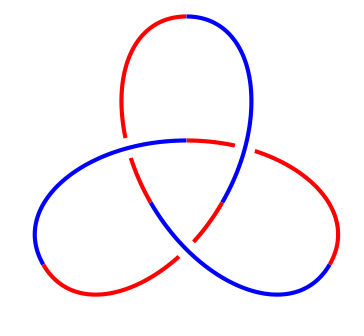
\includegraphics[width=0.22\linewidth]{3_1}}
        \hfill
        \subfloat[$5_1$ (cinquefoil)\label{fig:5-1}]{
            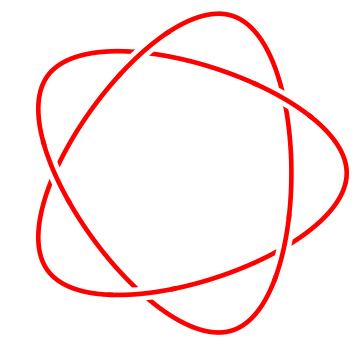
\includegraphics[width=0.22\linewidth]{5_1}}
        \hfill
        \subfloat[$5_2$ (cinquefoil twist)\label{fig:5-2}]{
            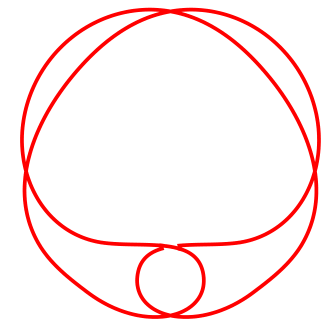
\includegraphics[width=0.22\linewidth]{5_2}}
        \hfill
        \subfloat[$6_1$ (stevedore)\label{fig:6-1}]{
            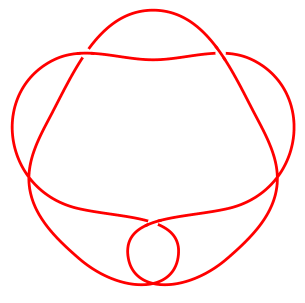
\includegraphics[width=0.22\linewidth]{6_1}}
        \caption{Canonical knot gallery.}
        \label{fig:knot-gallery}
        \end{figure}





    Each knot can be parametrized on a torus with major radius $R$ and minor radius $r$.
    The core tube of radius $r_c$ supports a tangential swirl velocity $\vswirl$, defining the \emph{Swirl Clock} $\SwirlClock$.

    A defining feature is that all these knots possess a \emph{central hole} threaded by a straight axis (taken as the $z$-axis).
    This axis is the ``fabric line'' of flat space: it is the singularity in the analytic swirl potential.


        \begin{figure}[t]
        \centering
        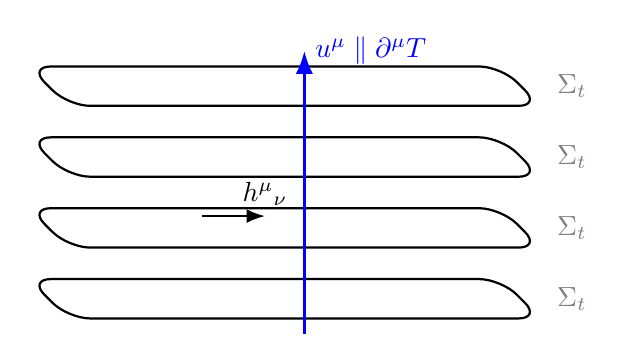
\begin{tikzpicture}[scale=1.0,>=Latex]
            % Stacked leaves
        \foreach \y in {0,0.9,1.8,2.7}{
            \draw[rounded corners=8pt,thick] (-3,\y) -- (3,\y) -- (2.5,\y+0.5) -- (-3.5,\y+0.5) -- cycle;
            \node[gray] at (3.4,\y+0.25) {$\Sigma_{t}$};
        }
% Foliation vector u
        \draw[->,very thick,blue] (0,-0.2) -- (0,3.4) node[right] {$u^\mu \parallel \partial^\mu T$};
% Projection hint
        \draw[->,thick] (-1.3,1.3) -- (-0.5,1.3) node[above] {$h^\mu{}_\nu$};
        \end{tikzpicture}
        \caption{Preferred foliation by the clock field $T(x)$ with unit timelike $u^\mu$, and spatial projector $h_{\mu\nu}=g_{\mu\nu}+u_\mu u_\nu$.}
        \end{figure}


% ============================
% Figure: Trefoil + central axis + circulation loops (clean, layered)
% ============================
        \begin{figure}[htbp]
        \centering
% Preamble requirement (once per document):
% \usetikzlibrary{decorations.markings}

        \begin{tikzpicture}[scale=0.90, line cap=round, line join=round]
% ------------------------
% Parameters
% ------------------------
        \def\R{3.20}      % major radius (to center of tube)
        \def\rtube{0.95}  % tube radius (for planar projection amplitude)
        \def\Rin{\R-\rtube}
        \def\Rout{\R+\rtube}

% ------------------------
% Styles
% ------------------------
        \tikzset{
            axisline/.style={->, line width=0.6pt, black!70},
            annulusfill/.style={fill=gray!10, even odd rule},
            annulusline/.style={draw=gray!55, line width=0.6pt},
            corecircle/.style={draw=black!70, line width=0.8pt},
            outercircle/.style={draw=black!60, line width=0.8pt, dash pattern=on 3pt off 2pt},
            labelbox/.style={fill=white, draw=black!20, rounded corners=2pt, inner sep=3pt},
            knotunder/.style={draw=blue!45!black, line width=1.4pt},
            knotover/.style={
                draw=blue!80!black, line width=1.4pt,
                preaction={draw=white, line width=3.2pt, line cap=round}
            },
            knotarrows/.style={
                postaction={decorate},
                decoration={
                    markings,
                    mark=at position 0.18 with {\arrow{Latex}},
                    mark=at position 0.52 with {\arrow{Latex}},
                    mark=at position 0.86 with {\arrow{Latex}}
                }
            }
        }

% ------------------------
% Axes (x-y plane view)
% ------------------------
        \draw[axisline] (-0.3,0) -- (6.8,0) node[below right] {$x$};
        \draw[axisline] (0,-3.6) -- (0,3.6) node[left] {$y$};

% Central rotational axis marker (z comes out of plane at origin)
        \fill[black] (0,0) circle(2pt);
        \node[below left] at (0,0) {\small central axis ($z$)};

% ------------------------
% Torus annulus (projection band)
% ------------------------
        \fill[annulusfill] (0,0) circle (\Rout) (0,0) circle (\Rin);
        \draw[annulusline] (0,0) circle (\Rin);
        \draw[annulusline] (0,0) circle (\Rout);
        \node[labelbox, align=left] at (\R,-2.35) {\footnotesize torus annulus $[R-\!r,\,R+\!r]$};

% ------------------------
% Circulation test loops in z=0 plane
% ------------------------
        \foreach \RR in {2.10, 2.60, 3.20} {
            \draw[corecircle] (0,0) circle (\RR);
        }
        \node[labelbox] at (2.10, 1.25) {\(\Gamma \approx -3\,\kappa\)};
        \node[labelbox] at (2.60,-1.25) {\(\Gamma \approx -3\,\kappa\)};
        \node[labelbox] at (3.20, 1.25) {\(\Gamma \approx -3\,\kappa\)};

% Outside loop ~ 0
        \draw[outercircle] (0,0) circle (4.6);
        \node[labelbox] at (4.6,-1.25) {\(\Gamma \approx 0\)};

% ------------------------
% Trefoil T(2,3) projection on torus: parametric planar curve
% x(θ) = (R + r cos(3θ)) cos θ
% y(θ) = (R + r cos(3θ)) sin θ
% Over/under decided by sign of z(θ) = r sin(3θ):
%   sin(3θ) > 0  => "over" segments
%   sin(3θ) < 0  => "under" segments
% We split [0, 2π] at θ = k·π/3.
% ------------------------
% parameters (numeric, no units)
        \def\R{3.20}
        \def\rtube{0.95}

% helper functions (degrees)
        \tikzset{
            declare function={
                Rx(\ang)= (\R + \rtube*cos(3*\ang))*cos(\ang);
                Ry(\ang)= (\R + \rtube*cos(3*\ang))*sin(\ang);
            }
        }

% --- UNDER segments first (behind) ---
        \draw[knotunder, samples=240, smooth, variable=\ang, domain=60:120]
        plot ({Rx(\ang)}, {Ry(\ang)});
        \draw[knotunder, samples=240, smooth, variable=\ang, domain=180:240]
        plot ({Rx(\ang)}, {Ry(\ang)});
        \draw[knotunder, samples=240, smooth, variable=\ang, domain=300:360]
        plot ({Rx(\ang)}, {Ry(\ang)});

% --- OVER segments (on top) ---
        \draw[knotover, knotarrows, samples=240, smooth, variable=\ang, domain=0:60]
        plot ({Rx(\ang)}, {Ry(\ang)});
        \draw[knotover, knotarrows, samples=240, smooth, variable=\ang, domain=120:180]
        plot ({Rx(\ang)}, {Ry(\ang)});
        \draw[knotover, knotarrows, samples=240, smooth, variable=\ang, domain=240:300]
        plot ({Rx(\ang)}, {Ry(\ang)});



% ------------------------
% Caption note inside canvas
% ------------------------
        \node[align=left, labelbox, anchor=south east] at (6.6,3.4) {\footnotesize
        Trefoil \(3_1\) (torus-knot projection)\\
        meridional winding \(q=3\)\\
        \(\Rightarrow\ \Gamma=\mathrm{Lk}\cdot\kappa=\pm 3\,\kappa\)
        };
        \end{tikzpicture}

        \caption{Trefoil knot with central axis and circulation loops in the \(z{=}0\) plane.
        Loops whose spanning disk intersects the filament within the torus annulus measure a plateau \(\Gamma=\mathrm{Lk}\cdot\kappa=\pm 3\,\kappa\) (sign by orientation).
        Loops outside the annulus do not enclose the filament and give \(\Gamma\approx 0\).}
        \label{fig:trefoil_axis_plateau_clean}
        \end{figure}



\section{Cauchy Integral and Circulation Quantization}
        Let $C$ be a closed loop in the $x$–$y$ plane encircling the $z$-axis. For an analytic swirl potential $W(z)=\Phi+i\Psi$ in a simply connected region,
        \begin{equation}
        \oint_C \vswirl \cdot d\mathbf{l} =
        \begin{cases}
        0, & \text{if no singularity inside,}\\[4pt]
        2\pi i\, \mathrm{Res}\!\left(\frac{dW}{dz}, z=0\right), & \text{if the axis is enclosed.}
        \end{cases}
        \end{equation}
        In SST we identify the residue with a circulation quantum $\kappa$. Independently of the complex-potential language, Kelvin’s theorem fixes circulation on any material loop; both viewpoints agree on the integer plateau:
        \begin{equation}
        \Gamma_C = n\,\kappa \quad \text{if the loop links $n$ times with the core.}
        \end{equation}

        \begin{tcolorbox}[title=\textbf{Canonical identification of $\kappa$ (SST)}]
        We adopt the equivalence
        \[
            \boxed{\;\kappa \equiv \frac{h}{m_{\text{eff}}} \;=\; 2\pi\, r_c\, v_c\;}
        \]
        which gives a direct bridge between the quantum of circulation and core kinematics. Hence
        \[
            m_{\text{eff}} \;=\; \frac{h}{2\pi r_c v_c}\,.
        \]
        \textbf{Numerics (SI):} with $r_c=\qty{1.40897017e-15}{m}$ and $v_c=\lVert \mathbf{v}_{\swirlarrow}\rVert=\qty{1.09384563e6}{m/s}$,
        \[
            \kappa=2\pi r_c v_c=\qty{9.6836192e-9}{m^2/s},\qquad
            m_{\text{eff}}=\frac{h}{\kappa}=\qty{6.842555e-26}{kg}\approx\qty{38.384}{GeV/c^2}.
        \]
        \end{tcolorbox}

        \noindent\emph{Status/limits:} Dimensions are consistent ($[\kappa]=L^2T^{-1}$). For loops whose spanning disk intersects the torus annulus of the filament, $\Gamma$ plateaus at $n\kappa$; for loops entirely outside, $\Gamma\approx 0$ (as illustrated in Fig.~\ref{fig:fourpanel-3D-cartoon}).

        \begin{tcolorbox}[title=\textbf{Swirl–EM correspondence (operational note)}]
        In the Canon’s swirl–EM mapping, time-varying core areal density acts as a “source” via a term of the form $b^{\swirlarrow}=G^{\swirlarrow}\,\partial_t \varrho^{\swirlarrow}$, providing a handle for experimental couplings. Dynamics on the central line that modulate $\varrho^{\swirlarrow}$ can therefore seed measurable EM-like responses without curving space, consistent with the flat-space treatment used here.
        \end{tcolorbox}


\section{Composite Baryon Tubes}
    Inside baryons, three quark knots (e.g.\ $5_2$, $5_2$, $6_1$ see fig~\ref{fig:5-2},~\ref{fig:6-1}) meet at a Y-shaped junction, forming a single composite swirl tube (see fig~\ref{fig:baryon_composite_tube}).



\begin{figure}[htbp]
    \centering
    \subfloat[Top view of 3 quarck knots\label{fig:baryon}]{
        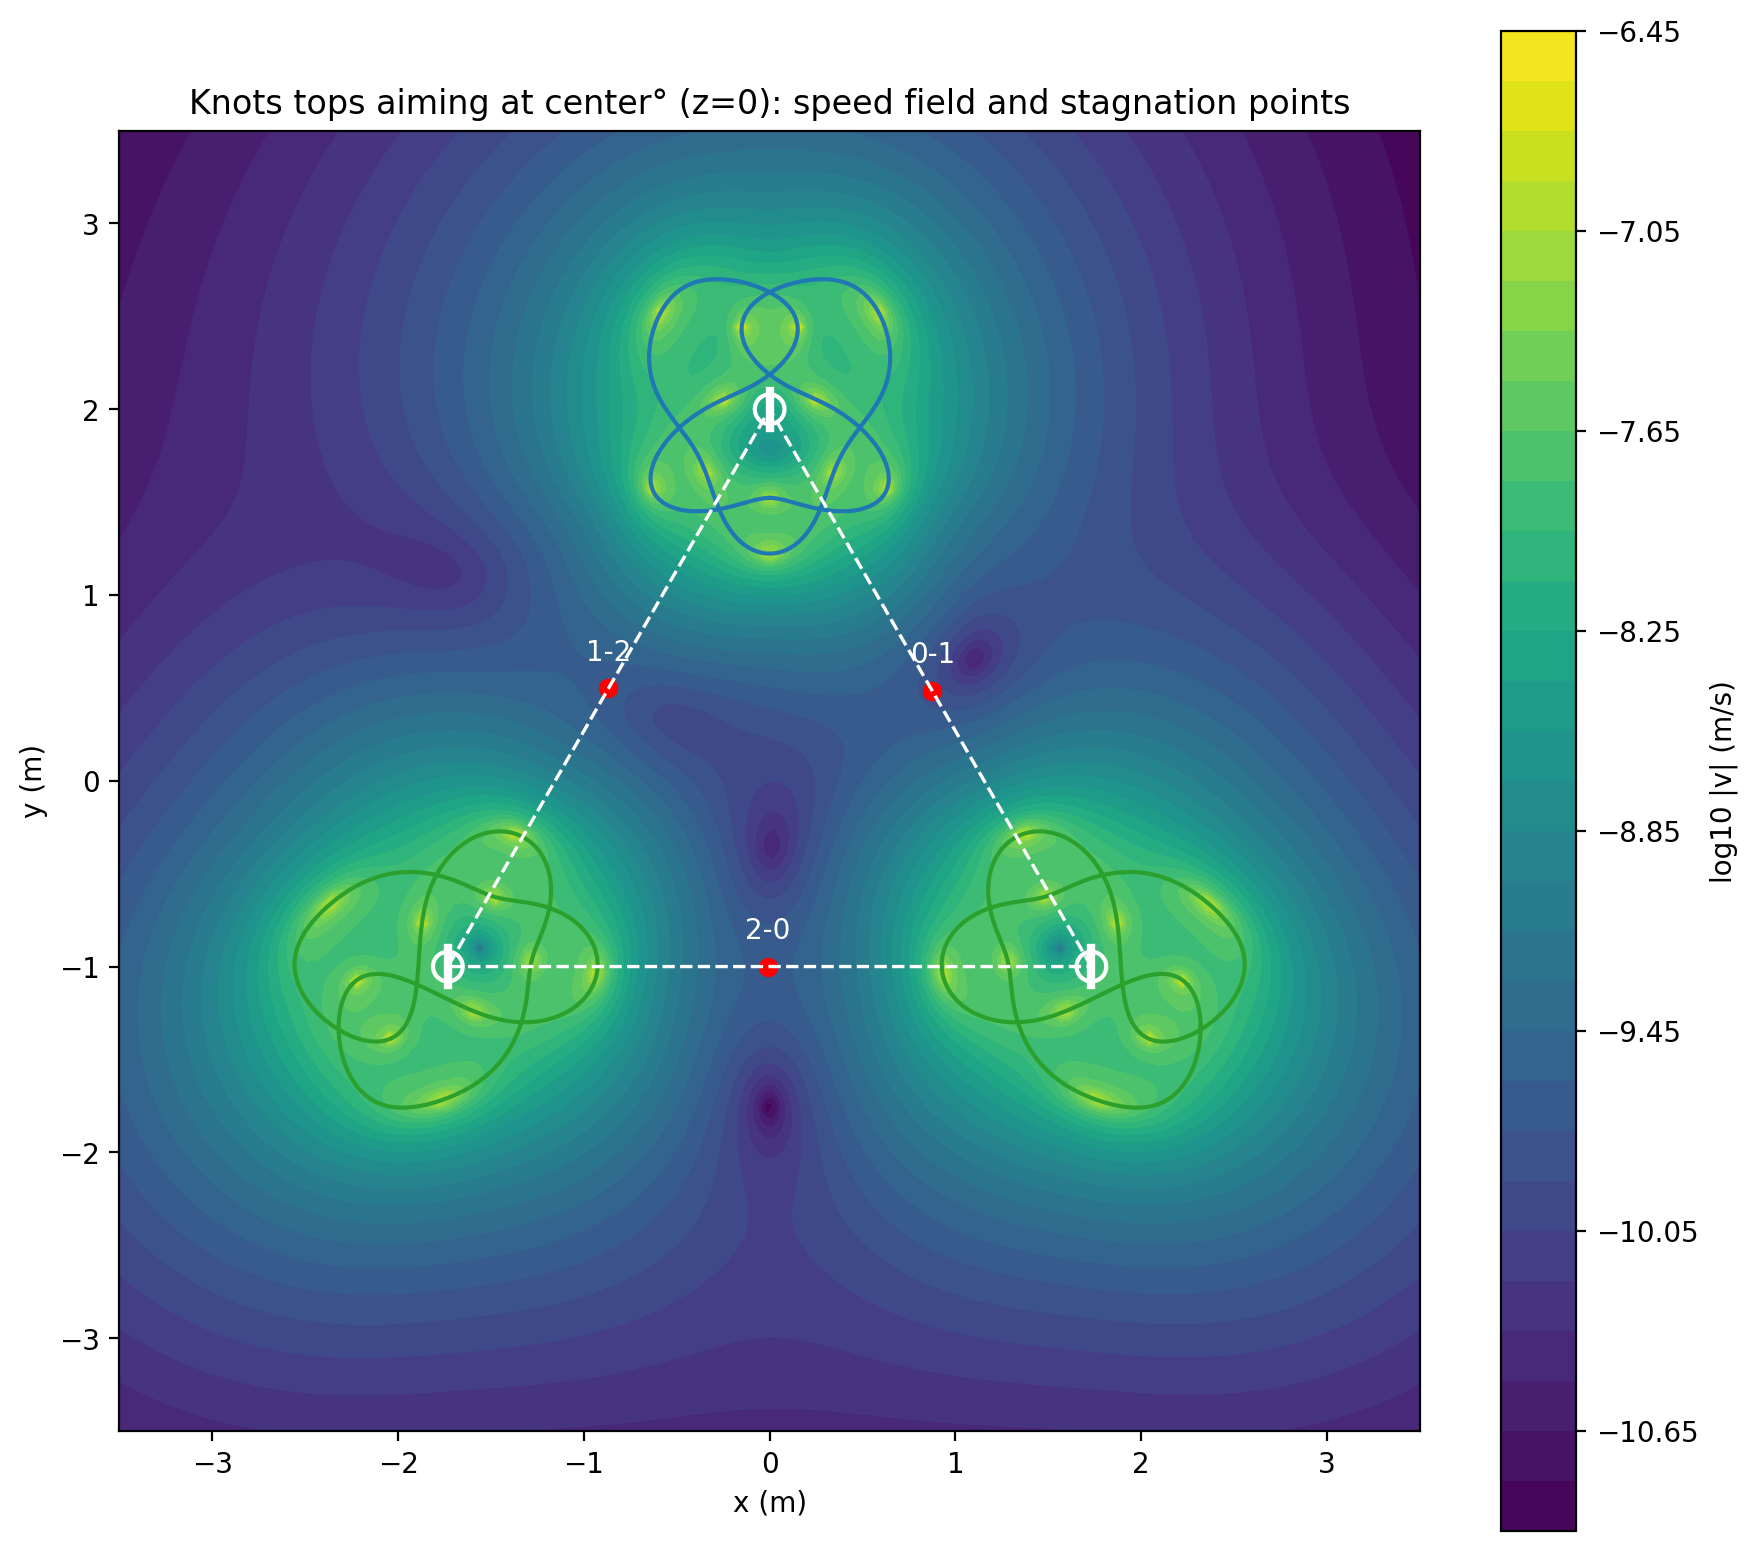
\includegraphics[width=0.3\linewidth]{sst_three_knot_180_speed_stagnation}}
    \subfloat[3D view of 3 quarck knots\label{fig:baryon3d1}]{
        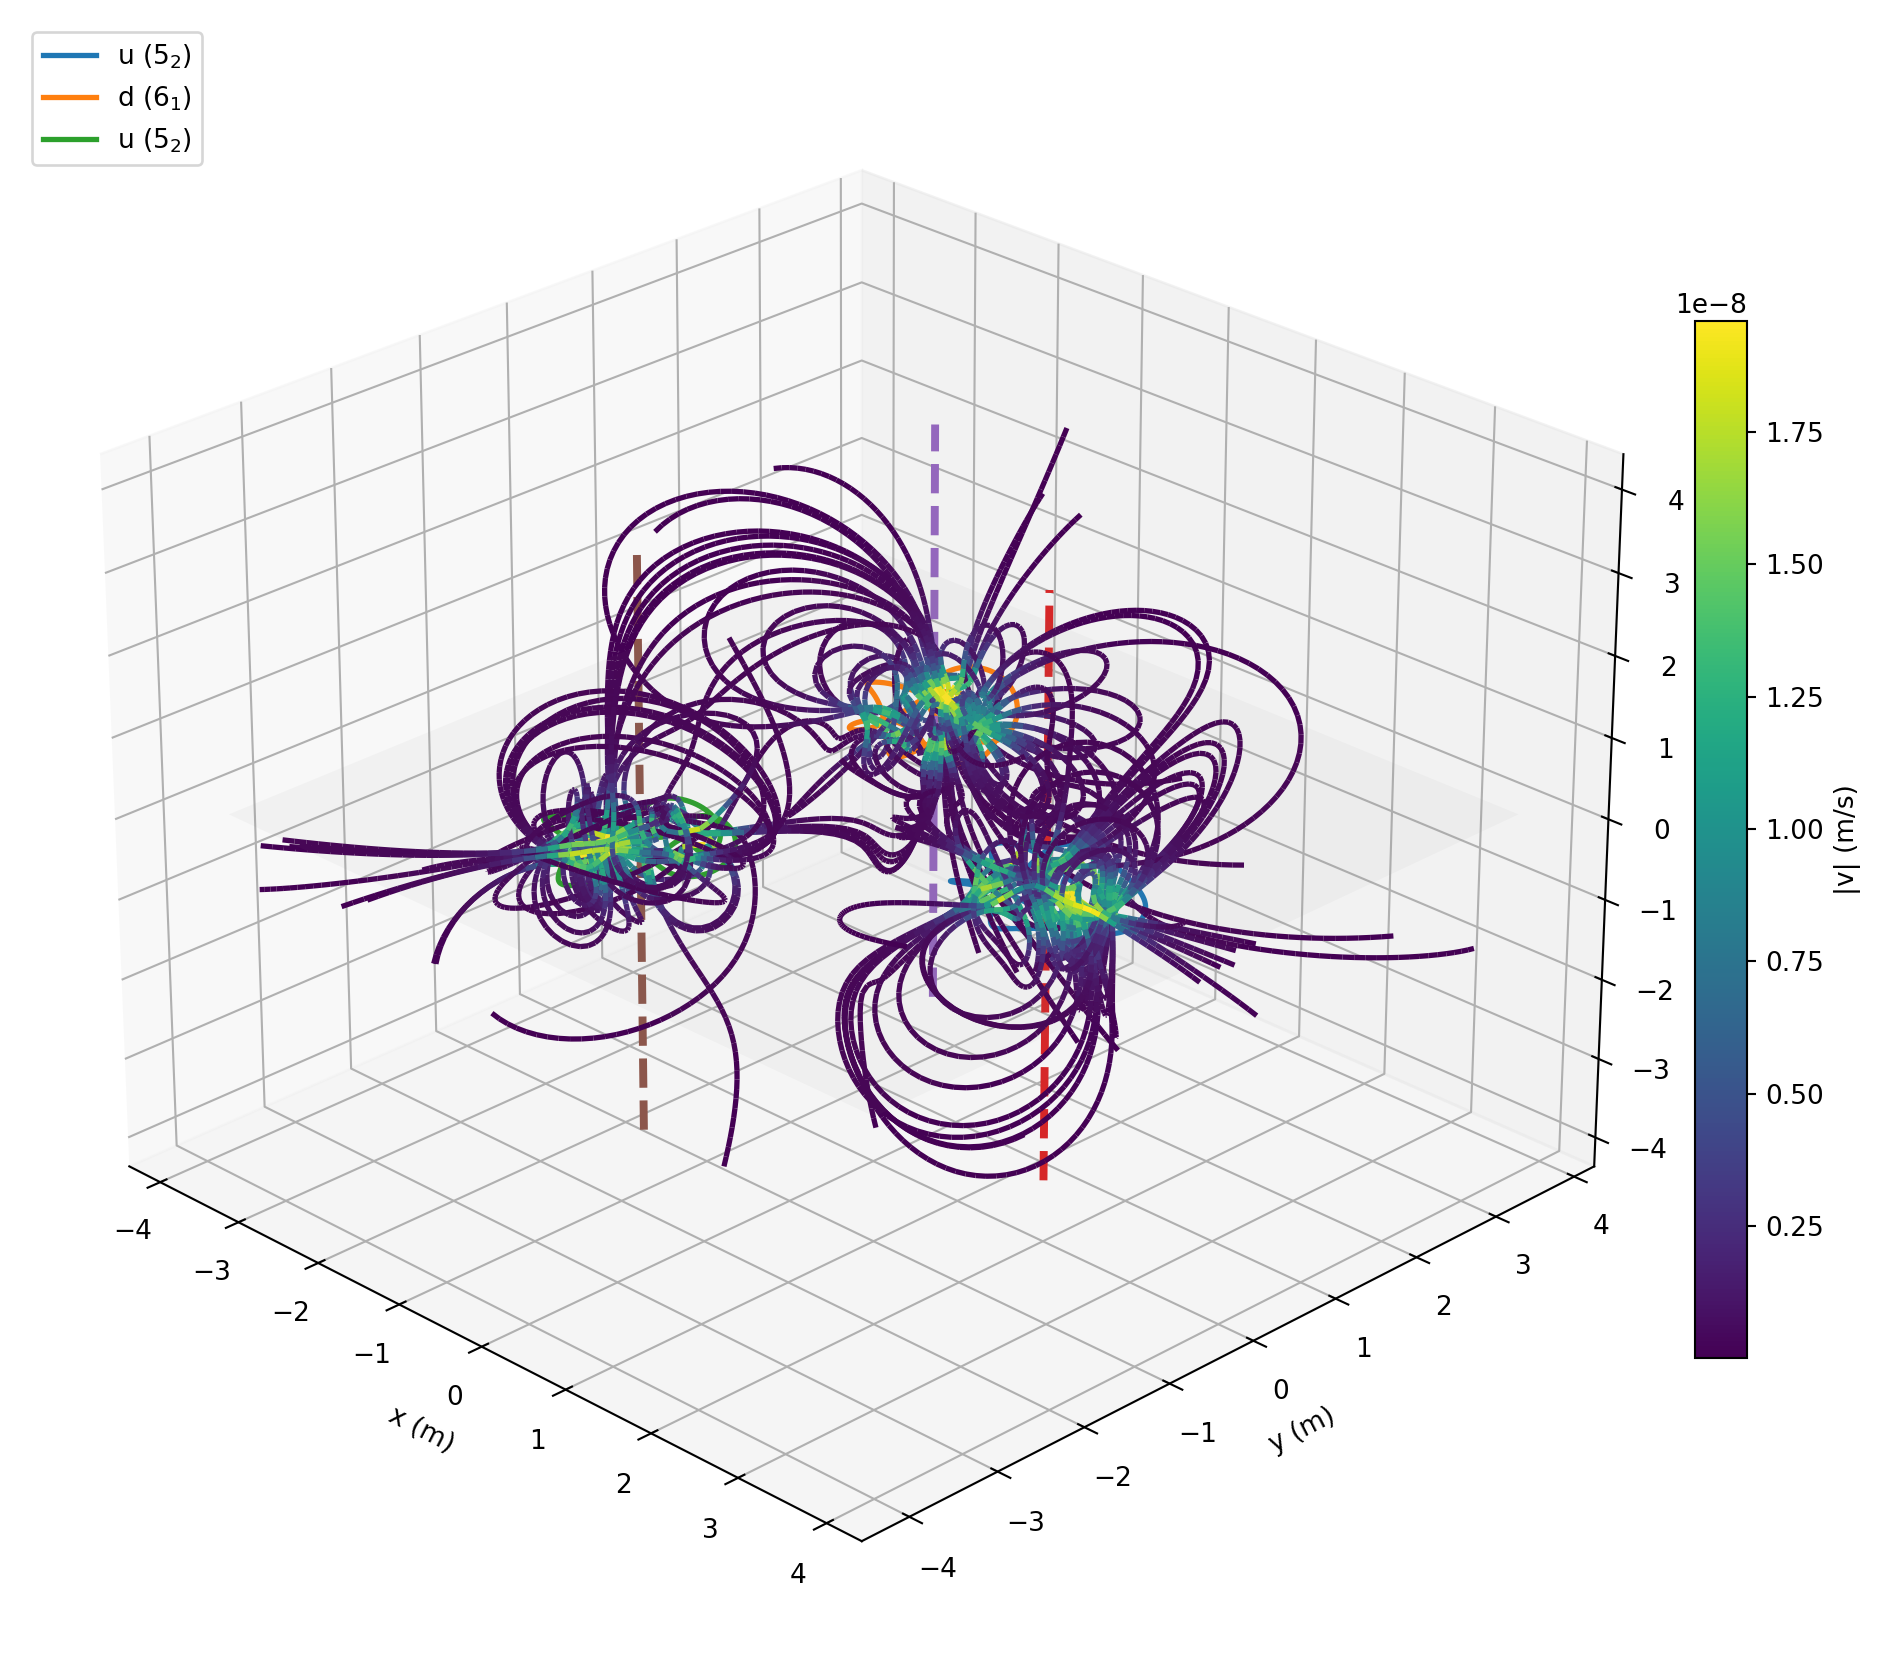
\includegraphics[width=0.3\linewidth]{sst_three_knot_3d_streamlines_colored_ULTRALIGHT}}
    \subfloat[Composite tube\label{fig:baryon_composite_tube}]{



% ============================
% Figure 2 (rotated): Baryon composite tube merging vertically on the z-axis
% ============================

        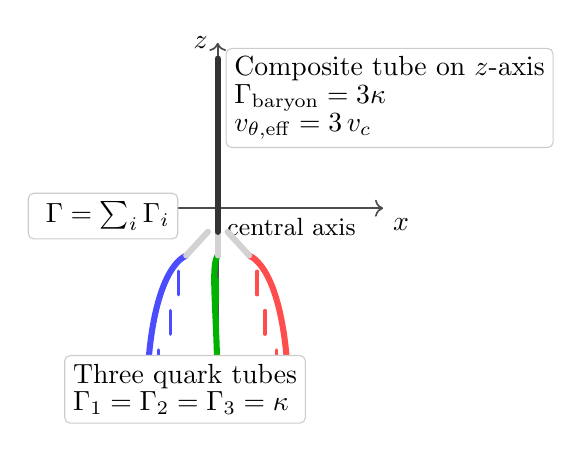
\begin{tikzpicture}[scale=0.5, line cap=round, line join=round]

% ---------- Styles ----------
        \tikzset{
            axisline/.style={draw=black!70, line width=0.6pt},
            tube/.style={draw, line width=2.2pt, rounded corners=2pt},
            vline/.style={draw, line width=1.2pt},
            labelbox/.style={fill=white, draw=black!20, rounded corners=2pt, inner sep=3pt}
        }

% ---------- Axes ----------
        \draw[axisline, ->] (0,-5.2) -- (0,4.2) node[left] {$z$};
        \draw[axisline, ->] (-4.2,0) -- (4.2,0) node[below right] {$x$};

% Central axis marker
        \fill (0,0) circle (2pt);
        \node[below right] at (0,0) {\small central axis};

% ---------- Three incoming quark tubes (from -z, merging to z-axis) ----------
% Left (blue)
        \draw[tube, blue!70]
        (-1.8,-5.0) .. controls + (0,2.1) and +(-0.6,-0.3) .. (-0.8,-1.2);
% Center (green)
        \draw[tube, green!70!black]
        (0.0,-5.0) .. controls + (0,2.3) and +(-0.2,-0.3) .. (0.0,-1.2);
% Right (red)
        \draw[tube, red!70]
        (1.8,-5.0) .. controls + (0,2.1) and +(0.6,-0.3) .. (0.8,-1.2);

% ---------- Y-junction region into the central tube ----------
        \draw[tube, gray!35] (-0.8,-1.2) -- (-0.25,-0.6);
        \draw[tube, gray!35] ( 0.0,-1.2) -- ( 0.0,-0.6);
        \draw[tube, gray!35] ( 0.8,-1.2) -- ( 0.25,-0.6);

% ---------- Composite tube along +z on the central axis ----------
        \draw[tube, black!80]
        (0.0,-0.6) .. controls +(0,0.9) and +(0,-0.9) .. (0.0,3.8);

% ---------- Swirl/flow direction tick marks ----------
% Incoming (upwards along +z)
        \foreach \x/\z in {-1.5/-4.2, -1.2/-3.2, -1.0/-2.2}{
            \draw[vline, blue!70] (\x,\z) -- ++(0,0.6);
        }
        \foreach \x/\z in {0.0/-4.4, 0.0/-3.4, 0.0/-2.4}{
            \draw[vline, green!70!black] (\x,\z) -- ++(0,0.6);
        }
        \foreach \x/\z in {1.5/-4.2, 1.2/-3.2, 1.0/-2.2}{
            \draw[vline, red!70] (\x,\z) -- ++(0,0.6);
        }
% Composite (upwards along +z)
        \foreach \z in {-0.2, 0.8, 1.8, 2.8}{
            \draw[vline, black!80] (0.0,\z) -- ++(0,0.8);
        }

% ---------- Labels ----------
        \node[align=left, labelbox, anchor=west] at (-3.9,-4.6) {Three quark tubes\\[-2pt]
        \(\Gamma_1=\Gamma_2=\Gamma_3=\kappa\)};
        \node[align=left, labelbox, anchor=west] at (0.2,2.8) {Composite tube on \(z\)-axis\\[-2pt]
        \(\Gamma_{\text{baryon}}=3\kappa\)\\[-2pt]
        \(v_{\theta,\mathrm{eff}}=3\,v_c\)};
        \node[align=left, labelbox, anchor=east] at (-1,-0.2) { \(\ \Gamma=\sum_i \Gamma_i\)};

        \end{tikzpicture}
    }
        \caption{Baryon core as a \emph{composite swirl tube}. Three quark tubes (bottom) join via a Y-junction into a single tube along $+z$. Circulation adds linearly, $\Gamma_{\rm baryon}=3\kappa$, hence $v_{\theta,\rm eff}=\Gamma_{\rm baryon}/(2\pi r_{\rm eff})$ with $r_{\rm eff}\approx r_c$ to leading order.}
    \label{fig:three-knot-gallery}
\end{figure}

    Each quark knot $i$ has circulation $\Gamma_i = \kappa$ around the central axis (Fig.~\ref{fig:baryon_composite_tube}).
        By Kelvin additivity,
        \begin{equation}
        \Gamma_{\mathrm{baryon}}=\Gamma_1+\Gamma_2+\Gamma_3=3\kappa.
        \end{equation}
        Since $\Gamma=2\pi r\,v_\theta$,
        \begin{equation}
        \boxed{\;
        v_{\theta,\mathrm{eff}}=\frac{\Gamma_{\mathrm{baryon}}}{2\pi\,r_{\mathrm{eff}}}
            =\frac{3\kappa}{2\pi\,r_{\mathrm{eff}}}\,,
            \;}
        \end{equation}
        with $r_{\mathrm{eff}}$ the effective core radius of the merged tube. In the thin-core, near-Rankine limit $r_{\mathrm{eff}}\approx r_c$ to leading order (so that $v_{\theta,\mathrm{eff}}\approx 3 v_c$ holds as a first-order estimate), while the deeper pressure well is set by the increased $\Gamma$.

        \paragraph{Swirl Clock scaling.}
        The Swirl Clock relation becomes
        \begin{equation}
        dt_{\mathrm{local}} = dt_\infty \sqrt{1 - \frac{(3 v_c)^2}{c^2}},
        \end{equation}
        predicting a more pronounced local time dilation, consistent with the larger rest mass of baryons relative to single quark knots.

            \emph{Analogy (for intuition).} Three equal water whirls feed one outlet: the hole may widen slightly, but the combined spin deepens the whirl and speeds the rim roughly threefold.

%
%%-------------------------------------------
%% 4-panel cartoon (same scale / same view)
%%-------------------------------------------
%\begin{figure}[htbp]
%\centering
%
%% -------- helper macro: one panel --------------
%% args: #1 = loop radius, #2 = ON/OFF style, #3 = caption text under panel
%\newcommand{\OnePanel}[3]{%
%    \begin{tikzpicture}[x=1cm,y=1cm,scale=0.60]
%    % parameters (shared across all panels)
%    \def\R{3.2}   % major radius (center of torus band)
%    \def\r{1.1}   % half-thickness of torus band
%    \def\tilt{0.55}% yscale to hint 3D tilt of torus
%    \def\RL{#1}   % test loop radius
%
%    % axes (same in all panels)
%    \draw[axes,->] (-0.25,0) -- (6.8,0) node[below right] {$x$};
%    \draw[axes,->] (0,-3.0) -- (0,3.0) node[left] {$y$};
%
%    % central axis marker (z coming out of page)
%    \fill (0,0) circle(2pt);
%    \node[below left] at (0,0) {\footnotesize central axis ($z$)};
%
%    % --- torus "band" with a little 3D hint (tilted annulus) ---
%    % outer and inner tilted ellipses (yscale = tilt)
%    \begin{scope}[yscale=\tilt]
%    \draw[very thick, gray!40] (0,0) circle (\R+\r);
%    \draw[very thick, gray!40] (0,0) circle (\R-\r);
%    % faint fill between ellipses for depth cue
%    \path[fill=gray!10,draw=none] (0,0) circle (\R+\r);
%    \clip (0,0) circle (\R+\r);
%    \fill[white] (0,0) circle (\R-\r);
%    \end{scope}
%
%    % --- schematic trefoil projection with over/under cues ---
%    % front arc (solid), back arc (dashed + lighter) to hint 3D crossing
%    % This is a clean cartoon, not exact geometry.
%    % Back (far) lobe:
%    \draw[knotline, dashed, opacity=0.35]
%    plot[smooth cycle, tension=0.9]
%    coordinates {
%        ({\R+0.2},  0.10)
%        ({\R-0.4},  0.95)
%        ({\R+0.6},  0.85)
%        ({\R+0.3}, -0.9)
%        ({\R-0.9}, -1.05)
%    };
%    % Front (near) lobe with arrows (swirl direction)
%    \draw[knotline]
%    plot[smooth cycle, tension=0.9]
%    coordinates {
%        ({\R},     0.00)
%        ({\R-0.6}, 1.00)
%        ({\R+0.8}, 0.80)
%        ({\R+0.4},-1.00)
%        ({\R-0.8},-1.20)
%    };
%    % flow arrows along the visible lobe
%    \foreach \t/\L in {0/0.35, 60/0.35, 180/0.35}{
%        \draw[looparrow, blue!70]
%        ({\R+0.7*cos(\t)},{0.1+0.9*sin(\t)}) --
%        ++({0.7*cos(\t+25)*\L},{0.7*sin(\t+25)*\L});
%    }
%
%% --- test loop (the circulation contour) ---
%    \draw[#2] (0,0) circle (\RL);
%
%    % panel caption (under)
%    \node at (3.0,-2.7) {\small #3};
%    \end{tikzpicture}%
%}
%
%% --------- lay out four panels on one row ----------
%\OnePanel{0.55}{testloopOFF}{(a)\; very small loop $\Rightarrow\ \Gamma=0$}\hspace{0.9cm}
%\OnePanel{2.65}{testloopON}{(b)\; inside torus band $\Rightarrow\ \Gamma=-3\,\kappa$}\hspace{0.9cm}
%\OnePanel{3.25}{testloopON}{(c)\; still inside band $\Rightarrow\ \Gamma=-3\,\kappa$}\hspace{0.9cm}
%\OnePanel{4.60}{testloopOFF}{(d)\; far outside $\Rightarrow\ \Gamma\approx 0$}
%
%\caption{Four identical-scale, top-down panels. The gray tilted annulus hints at the torus where the trefoil lives (donut seen at an angle).
%The blue curve is a schematic trefoil; dashed parts are “behind” (3D cue).
%The green \textbf{test loops} (b,c) lie \emph{within} the torus band and measure the plateau \(\Gamma=\mathrm{Lk}\cdot\kappa=\pm 3\,\kappa\) (sign by orientation).
%Red loops (a,d) do not link the filament \(\Rightarrow \Gamma\approx 0\).}
%\label{fig:fourpanel-3D-cartoon}
%\end{figure}


\section{Swirl Gravity and Molecular Attraction}
Two composite tubes (e.g., two protons) sharing the same central line produce a combined circulation
\[
    \Gamma_{\mathrm{total}} = (3 \kappa)_{\mathrm{proton}} + (3 \kappa)_{\mathrm{proton}} = 6 \kappa,
\]
which deepens the shared pressure well and yields a stronger long-range attraction.
This explains why neutral molecules (e.g., H$_2$) still attract in Euclidean space: their baryon cores are connected by the same central line, and the resulting swirl gravity follows directly from the additive circulation.

\section{Conclusion}
Long-distance gravitational attraction in SST is a manifestation of topological quantization: chiral knots with central holes enforce non-vanishing circulation residues along a central line.
When multiple quark knots merge into a baryon, their circulations add linearly, forming a single composite tube with $3\kappa$ circulation.
This mechanism predicts the correct baryonic mass scaling and provides a flat-space explanation for molecular attraction.



\nocite{*}
\bibliographystyle{unsrt}
\bibliography{swirlgravity}






\end{document}
